\chapter{Extended model}\label{ch: extended_model}

\section{Model Rules}

In the extended model, toppling depends on the height difference between neighbouring sites rather than the height of an individual site. I set $k=4$, so a site transfers one grain of sand to each nearest neighbour whose height is at least four grains lower. All four directions are checked using the site's height before any grains are transferred.

Additionally, the height outside the grid is fixed at zero. Therefore, a boundary site with a height of at least four transfers one grain out of the system in each outward direction. Sites are processed row by row, from left to right within each row, and the process is repeated until the configuration is stable.

For example:

\[
\begin{pmatrix}
	0 & 4 & 1 \\
	1 & 4 & 0 \\
	0 & 0 & 0
\end{pmatrix}
\;\rightarrow\;
\begin{pmatrix}
	1 & 2 & 1 \\
	1 & 4 & 0 \\
	0 & 0 & 0
\end{pmatrix}
\;\rightarrow\;
\begin{pmatrix}
	1 & 2 & 1 \\
	1 & 2 & 1 \\
	0 & 1 & 0
\end{pmatrix}
\]

\section{Simulation and Results}
Similarly, I initialise a $50 \times 50$ matrix with all elements set to zero and initially set $T$=100,000. For the extended model, I simulate only one pile. I also set the random seed to 1643210 to ensure reproducibility. After each grain addition and the completion of all toppling activity, I record the average height, Topples, Area, Loss and Length, as in the basic model, for comparison. 

I first plot the average height against the number of grains added to estimate when the system reaches a steady state. After 100,000 grains have been added, the average height is still increasing, as shown in Figure~\ref{fig:avg_extend_height}. As the number of grains added to the system increases, the average height continues to rise, but at a decreasing rate. I generate a heat map to examine the spatial distribution of sand.

As shown in Figure~\ref{fig:extend_heat}, boundary sites contain fewer grains because their heights must remain below four after all toppling activity has ceased. Heights generally increase towards the centre, forming a flat-topped pyramid. I expect that further grain additions will raise the central region and reduce the size of the flat top, producing a shape closer to a pyramid. To investigate this, I add a further 100,000 grains of sand to the grid.

As shown in Figure~\ref{fig:avg_extend_height_2}, the average height levels off at approximately 26.5 after about 190,000 grain additions. Therefore, I exclude the first 190,000 records as burn-in.

\begin{figure}[!htbp]
	\centering
	\begin{minipage}{0.35\textwidth}
		\centering
		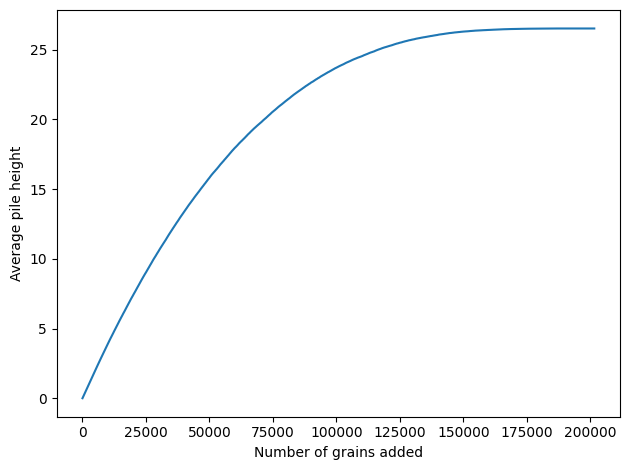
\includegraphics[width=\linewidth]{figures/avg_extend_height_2.png}
	\end{minipage}
	\hfill
	\begin{minipage}{0.35\textwidth}
		\centering
		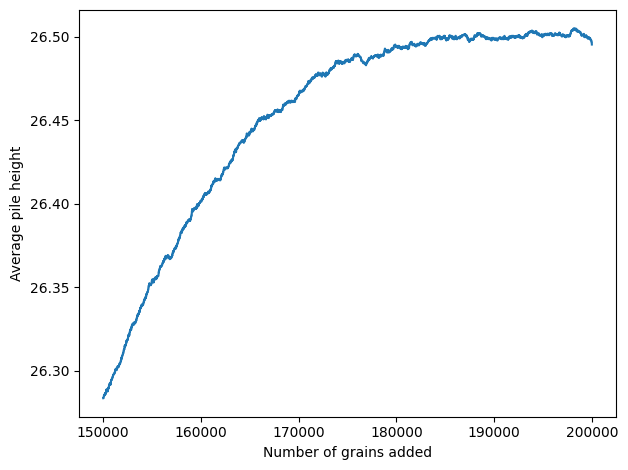
\includegraphics[width=\linewidth]{figures/avg_extend_height_2_zoom.png}
	\end{minipage}
	\caption{Average pile height against the number of grains added (left), with a zoomed-in view of the final stage (right).}
	\label{fig:avg_extend_height_2}
\end{figure}

\newpage

After a further 100,000 grains are added, the heat map shows a shape closer to a pyramid, consistent with the earlier prediction, as shown in Figure~\ref{fig:extend_heat_2}.
\begin{figure}[htbp]
	\centering
	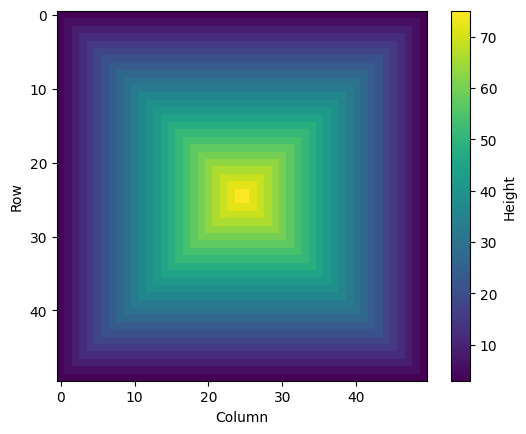
\includegraphics[width=0.5\textwidth]{figures/extend_heat_2.png}
	
	\caption{Spatial distribution of sand heights in the extended model.}
	\label{fig:extend_heat_2}
\end{figure}

After excluding the records collected during the burn-in period, I use the remaining records to plot the observed frequencies of the four avalanche properties and explore their distributions.

\begin{figure}[htbp]
	\centering
	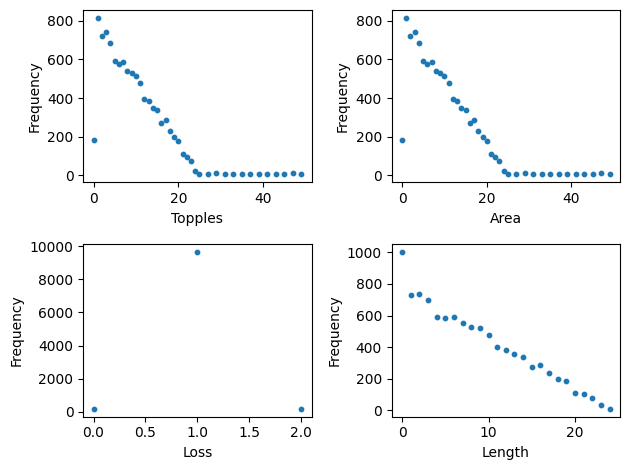
\includegraphics[width=0.6\textwidth]{figures/extend_linear.png}
	\caption{Observed frequencies of Topples, Area, Loss, and Length for one simulation of the extended model on linear axes.}
	\label{fig:extend_linear}
\end{figure}

As shown in Figure~\ref{fig:extend_linear}, the frequencies of Topples and Area decrease approximately linearly over the main range of positive values, with a small number of larger events forming a tail. Length also shows an approximately linear decreasing trend. Additionally, 9,622 of the 10,000 Loss values recorded after the burn-in period are equal to 1, while 185 are equal to 0 and 193 are equal to 2.